\documentclass[11pt]{article}
\usepackage{graphicx}
\usepackage{color}
\usepackage[utf8]{inputenc}
\usepackage[english]{babel}
\usepackage[a4paper,margin=1 in]{geometry}
\usepackage[backend=biber,style =
chem-acs,url=false,isbn=false,maxbibnames=90,articletitle,doi=false]{biblatex}
\usepackage[colorlinks=true,allcolors=blue]{hyperref}
\usepackage[version=3]{mhchem}
\usepackage{setspace}
\usepackage{longtable}
\usepackage{multirow}
\usepackage{booktabs}
\usepackage{lineno}
\addbibresource{Refs.bib}

\begin{document}
\linenumbers
\doublespacing

\title{Explicit and Mean-Field Models for Coverage-Dependent CO Adsorption on Pd(111)}

\author{John P. Clay,$^{a}$ Steven J. McDonough,$^{a}$ Kurt Frey,$^{a}$ Jeffrey P. Greeley,$^{b}$ Fabio H. Ribeiro,$^{b}$ \\ W. Nicholas Delgass,$^{b}$ and William F. Schneider$^{a,c}$\footnote{Corresponding author: wschneider@nd.edu, +1-574-631-8754}} 
\date{}
\maketitle
\noindent
{$^{a}$ Department of Chemical and Biomolecular Engineering. 
	        182 Fitzpatrick Hall. University of Notre Dame. Notre Dame, IN 46556. USA}\\
{$^{b}$ School of Chemical Engineering.
			480 Stadium Mall Drive. Purdue University. West Lafayette, IN 47907. USA}\\
{$^{c}$ Department of Chemistry and Biochemistry. 
			251 Nieuwland Science Hall. University of Notre Dame. Notre Dame, IN 46556.
			USA}\\

\newpage

\section*{Introduction}
\label{intro}
\subsection*{Highlight}
\label{highl}

%做了啥别人没做的?gcmc simulation 去 get binding energy impact

\begin{enumerate}
%\begin{singlespace}
\item Developed one,two,three site cluster expansion model for Pd(111)-CO system.

\item Extract coverage-dependent CO binding energy on Pd from finite temperature Monte Carlo simulation (GCMC).

\begin{equation}\label{gcmc}
\bar{E}_{\ce{CO}}(\theta,T) =\mu_{\ce{CO}}(\theta,T)+T \bar{S}_{\ce{CO}}(\theta,T)
\end{equation}

\begin{equation} \label{entropy_n_meanfield}
	\bar{S}_\text{CO}(\theta,T) = -k_B T \ln \left ( \frac{\theta}{n*(1-\theta)} \right )
\end{equation}

\item Obtain analytical expression of coverage dependent binding energy $\bar{E}(\theta)$.
\item Simulated CO TPD with analytical expression of $\bar{E}(\theta)$ consistent with experimental TPD. 

\begin{equation}\label{tpd}
r_\mathrm{Des}=-\frac{\partial \theta}{\partial T}={\nu *\theta}*\exp \left( \frac{\bar{E}_\mathrm{CO}(\theta)}{k_\mathrm{B} T} \right)
\end{equation}

%\end{singlespace}
\end{enumerate}

\subsection*{Justification}
\label{jus}
\begin{enumerate}
\item CO adsorption step is crucial in WGS reaction process. Adsorption site and adsorbates interaction can effect binding energy of CO. From volcano plot, binding enregy related to catalyst activity. Capturing binding energy will contribute to better prediction of temperature programmed desorption (TPD) spectra and even to reliable microkinetic model.

\item Conventionally, DFT method was used to compute binding energy with certain coverage and configuration, or fitting function for formation energy vs.\ coverage and then take derivative. But it would be impractical to compute binding energy of all coverages and configurations.

\item An alternative method to represent DFT energy is Cluster Expansion(CE). CE is a polynomial form that can express energy by given configuration. CE model can be trained by DFT database and once it reach convergence, CE will be used as Hamiltonian to perform Monte Carlo simulation. GCMC simulation take advantage of fixed chemical potential (${\mu}$), temperature (T) and number of particles(N), large supercell and metropolis algorithm until system reach to specified convergence.

\item Having analytical expression of $\bar{E}_{CO}(\theta)$ will be convenient to predict TPD spectra from equation \ref{tpd} with Euler forward integration.
\end{enumerate}

\subsection*{Guide To Reader}
\label{guide}

Here we combine cluster expansion and Grand Canonical Monte Carlo (GCMC) simulation to extract coverage-dependent binding energy of CO on Pd (111). We explore how different CE model impact binding energy with various temperature. Three model are used to fit simulation result to obtain analytical expression of binding energy with respect to coverage, piecewise\cite{Grabow2010}, activity \cite{Bajpai2020} and logistic\cite{Grabow2008}. Then simulated TPD can be generated by those model. We compare simulated TPD with experimental TPD \cite{Guo1989} to confirm our approach can accurately model TPD spectra.

\begin{align*}
\text{Piece-wise linear:} & \quad \overline{E}_{\ce{CO}}(\theta) = A \text{ for }\theta<C\text{  and }A+B(\theta-C)\text{ for } \theta\geq C\\
\text{Activity:} & \quad \overline{E}_{\ce{CO}}(\theta)  =A+B\left\{\frac{\lambda_{1}}{1+\lambda_{1}\theta}+\ln\left(\frac{1+\lambda_{2}\theta}{1+\lambda_{1}\theta}\right)+\theta\left[\frac{\lambda_{2}-\lambda_{1}}{(1+\lambda_{2}\theta)(1+\lambda_{1}\theta)}\right]\right\}\\
\text{Logistic:} & \quad \overline{E}_{\ce{CO}}(\theta)  =\frac{A}{B \exp (C \theta ) + D}\\
\end{align*}
\clearpage

\subsection*{Results and Discussion}
\label{result}
\subsubsection*{Pd(111) Surface}
\begin{figure} [ht]
\centering
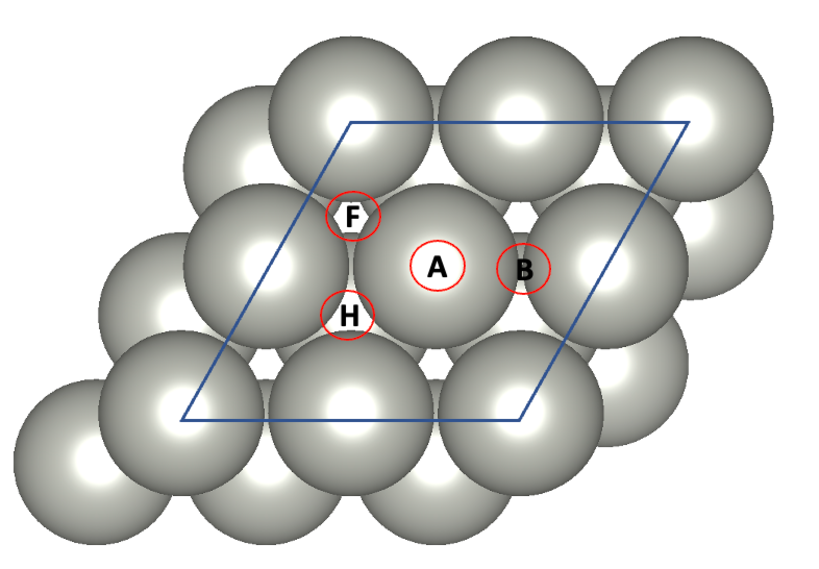
\includegraphics[width=10cm]{Figure/Pd.pdf}
\caption{Geometric relationship between FCC, HCP, and ATOP sites in the $(2 \times 2)$ supercell (black lines) on the (111) surface of a close-packed metal. (F) , (H), and (A) represent FCC, HCP,  ATOP sites, respectively.}
\label{Pd}
\end{figure}

\clearpage
\subsubsection*{Ground State}
\begin{figure} [h]
	\centering
	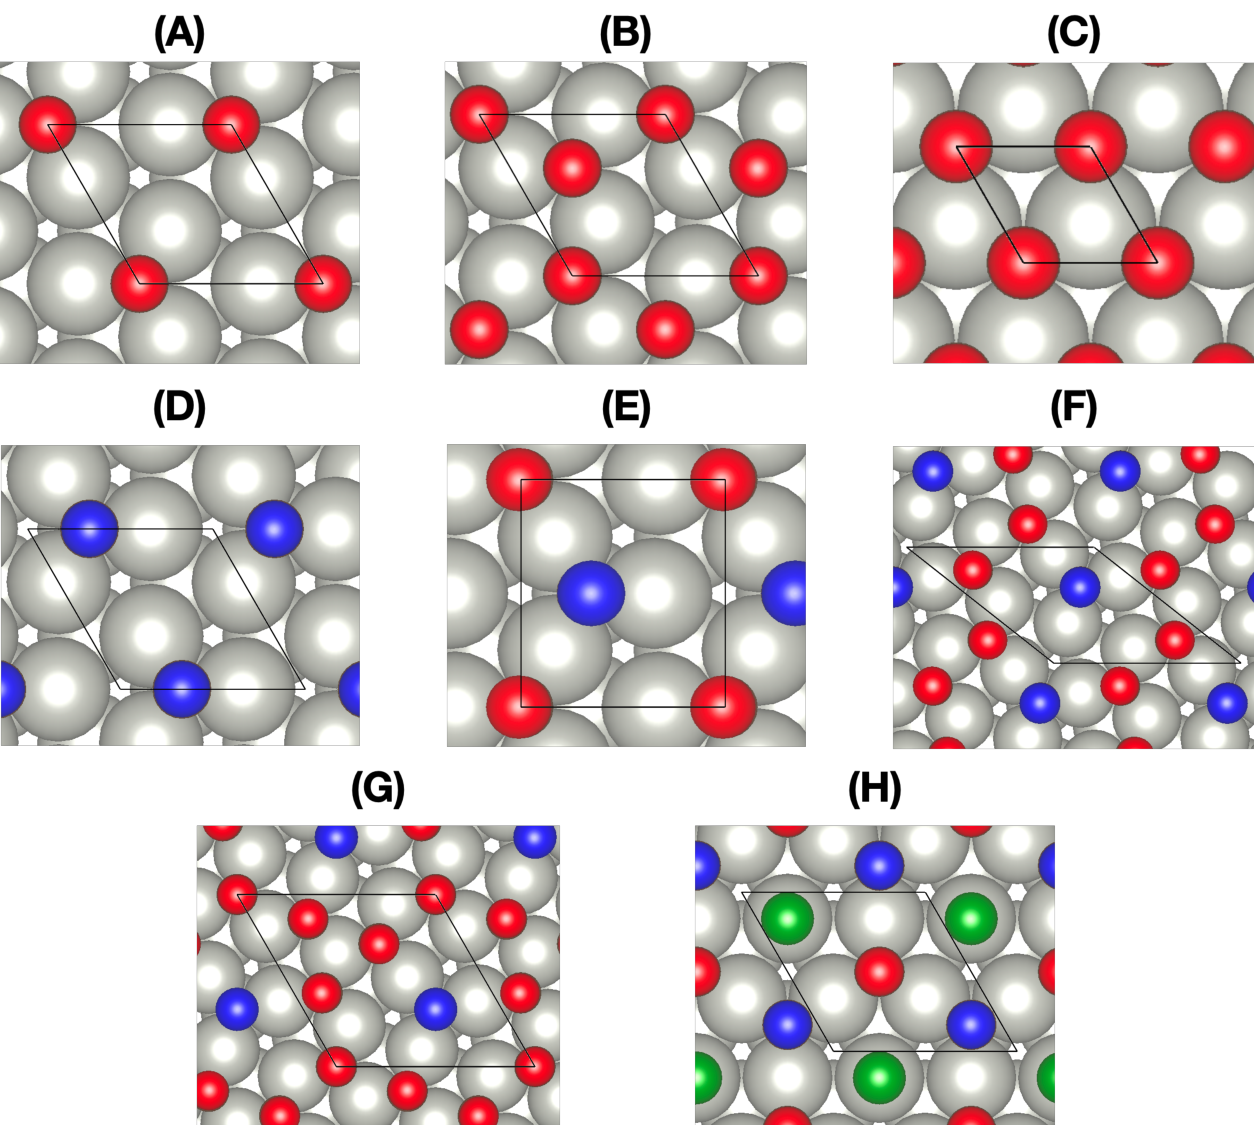
\includegraphics[width=13cm]{Figure/Gs1.pdf}
	\caption{Top view of computed ground state structures.  Red, blue and green correspond to FCC, HCP, and ATOP sites, respectively.  (A) 1/3 ML FCC, (B) 2/3 ML FCC, (C) 1 ML FCC, (D) $1/3$ ML HCP Hollow, (E) $1/2$ ML FCC/HCP, (F) $3/5$ ML FCC/HCP, (G) $5/7$ ML FCC/HCP, and (H) $3/4$ ML FCC/HCP/ATOP. Black lines represent the unit cell.}
	\label{GroundStates}
\end{figure}

\begin{table} [h]
	\caption{Geometric Data for the FCC Hollow Site Cluster Expansion Ground States.}  
	\centering
	\begin{tabular} {cc}
		\toprule
		Coverage (ML) & Geometry\\
		\midrule
		1/3                      & $(\sqrt{3}\times\sqrt{3})R30^\mathrm{o}-1$ \ce{CO} \\
		\\
		2/3     & $(\sqrt{3}\times\sqrt{3})R30^\mathrm{o}-2$ \ce{CO} \\
		\\
		1                        & ($1\times1$)-1 \ce{CO} \\
		\bottomrule
	\end{tabular}
	\label{1sitegs}
\end{table}

\begin{table} [h]
\caption{Geometric Data for the FCC and HCP Hollow Site Cluster Expansion Ground States.}
\centering
\begin{tabular} {c c}
\toprule
Coverage (ML) & Geometry\\
\midrule
1/3                   &  ($\sqrt{3}\times\sqrt{3})R30^\mathrm{o}-1$ \ce{CO} \\
\\
1/2  & c$(4\times2)-$2 \ce{CO}             \\
\\
3/5  & $|a|=|b|=7.399$ \AA, $\psi$=141.78$^\mathrm{o}$ \\
\\
5/7  & $|a|=|b|=7.399$ \AA, $\psi$=120.00$^\mathrm{o}$\\
\\
1                     &  ($1\times1)-$1 \ce{CO} \\
\bottomrule
\end{tabular}
\label{2sitegs}
\end{table}


\begin{table} [h]
	\caption{Geometric Data for the FCC, HCP Hollow, and Atop Site Cluster Expansion Ground States.}
	\centering
	\begin{tabular} {c c}
		\toprule
		Coverage (ML) & Geometry\\
		\midrule
		1/3                   &  ($\sqrt{3}\times\sqrt{3})R30^\mathrm{o}-1$ \ce{CO} \\
		\\
		1/2  & c$(4\times2)-$2 \ce{CO}             \\
		\\
		3/5  & $|a|=|b|=7.399$ \AA, $\psi$=141.78$^\mathrm{o}$ \\
		\\
		3/4  & $(2\times2)-3$ \ce{CO}\\
		\\
		1                     &  ($1\times1)-$1 \ce{CO} \\
		\bottomrule
	\end{tabular}
	\label{3sitegs}
\end{table}

\clearpage
\subsubsection*{Cluster Expansion}

\begin{figure} [h]
	\centering
	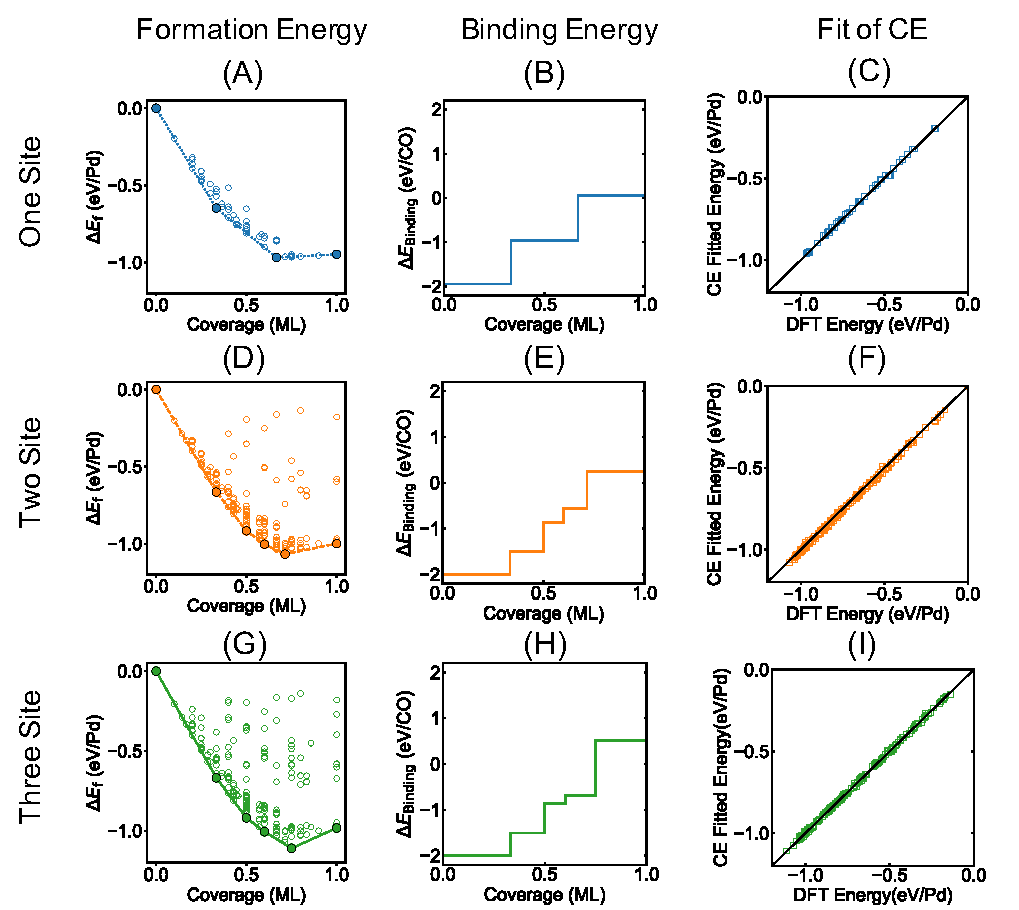
\includegraphics[width=15cm]{Figure/AllCE.pdf}
	\caption{First column: GGA-computed formation energies vs.\ coverage for FCC-only, FCC/HCP, and FCC/HCP/atop models from top to bottom. Middle column: differential binding energy vs.\ coverage for same three models. Last column: CE fitted vs.\ DFT-computed formation energies for same three models.}
	\label{All_CE}
\end{figure}

\begin{enumerate}
\item Figure \ref{All_CE} C compares the GGA-computed formation energies with the CE predictions.  The two-body-only CE fits the data with a cross validation score of 7.59 meV/\AA$^2$. Figure \ref{All_CE} A shows the DFT-computed formation energies.  The minimum energy hull has two ``kinks''  at $1/3$ and $2/3$ ML corresponding to a $(\sqrt{3} \times \sqrt{3})R30^\mathrm{o}-1$ \ce{CO}  (Figure \ref{GroundStates} A) and a $(\sqrt{3} \times \sqrt{3})R30^\mathrm{o}-2$ \ce{CO} configuration (Figure \ref{GroundStates} B), respectively.  Figure \ref{GroundStates} C includes for completeness the  $(1 \times 1)$ structure.  The slope of the formation energy hull is the 0~K  differential binding energy, $\bar{E}_{\ce{CO}}^{\text{FCC}}(\theta,0~\text{K})$, and is plotted in  Figure \ref{All_CE}  B.  The 0 K differential binding energy is constant to $1/3$~ML, up to which coverage each adsorbate can avoid any first nearest neighbor (1NN) interactions, steps up above $1/3$ ML as each new adsorbate accumulates three 1NNs, and steps up again to a positive value above $2/3$~ML, where each new adsorbate acquires 6 1NNs.

\item The inclusion of FCC and HCP sites together yields a richer formation energy hull, shown in Figure \ref{All_CE} D. The ground state at $1/3$~ML remains and has the same $(\sqrt{3} \times \sqrt{3})R30^\circ-1$ \ce{CO} structure, although as expected from the comparisons in Table \ref{1sitegs}, with CO in HCP sites (Figure~\ref{GroundStates} D).  A new ground state appears at $1/2$ ML in which half the CO occupy FCC and half HCP sites, each CO sublattice having c$(4\times2)$ symmetry (Figure~\ref{GroundStates} E).  In this configuration half the surface Pd have two CO in opposing (second nearest neighbor, 2NN) FCC and HCP sites and the other half have either a single FCC or HCP CO.  Another new ground state appears at $3/5$ ML (Figure~\ref{GroundStates} F) in which $2/3$ of the CO occupy FCC and $1/3$ HCP sites.  Here the FCC CO form chains of adjacent occupied sites like that in the $2/3$ ML FCC-only structure, with the chains separated by intervening rows of HCP CO.  The more dense $2/3$ ML FCC-only ground state disappears in the FCC/HCP system.  In its place appears a $5/7$ ML structure (Figure~\ref{GroundStates} G) in which $4/5$ of the CO occupy FCC and $1/5$ HCP sites.  The structure is more complex, but the 2NN FCC-HCP motif is retained.  At $1$ ML the FCC-only configuration is lower in energy than HCP-only; any mixed configuration would have high energy 1NN CO. As evident from Figure \ref{All_CE} D, many other configurations are close in energy to the ground state hull.  Figure \ref{All_CE} E plots the differential binding energy $\bar{E}_{\ce{CO}}^{\mathrm{F/H}}(\theta)$ extracted from the ground state hull.  Energies increase in more gradual steps than in the FCC-only model up to $5/7$ ML, where $\bar{E}_{\ce{CO}}^{\text{F/H}}(\theta)$ jumps to a strongly positive value.  Table \ref{2sitegs} summaries the structures for the ground states.

\item Figure \ref{All_CE} I shows a comparison of the DFT computed formation energies with the cluster expansion predicted formation energies. Figure~\ref{All_CE} G shows the DFT formation energies with the formation energy hull, where there are ``kinks'' at $1/3$, $1/2$, $3/5$, and $3/4$ ML, which correspond to the ground states. The ground states at $1/3$, $1/2$, $3/5$ and $1$ ML are the same ground states determined in by the FCC, and HCP Hollow site cluster expansion (Figure \ref{GroundStates} C-F). A new ground state at $3/4$ ML has CO adsorbed in a FCC Hollow, HCP Hollow and Atop site. Figure \ref{All_CE} H shows the 0 K differential binding energy, where there are steps at 0, $1/3$, $1/2$, $3/5$, and $3/4$ ML. At $3/4$ ML, the 0 K differential binding energy becomes positive, which is different from the previous models. Table \ref{3sitegs} reports the geometric configurations for the ground states
\end{enumerate}
 
\clearpage

\subsubsection*{GCMC Simulation Result}
\begin{figure} [h]
\centering
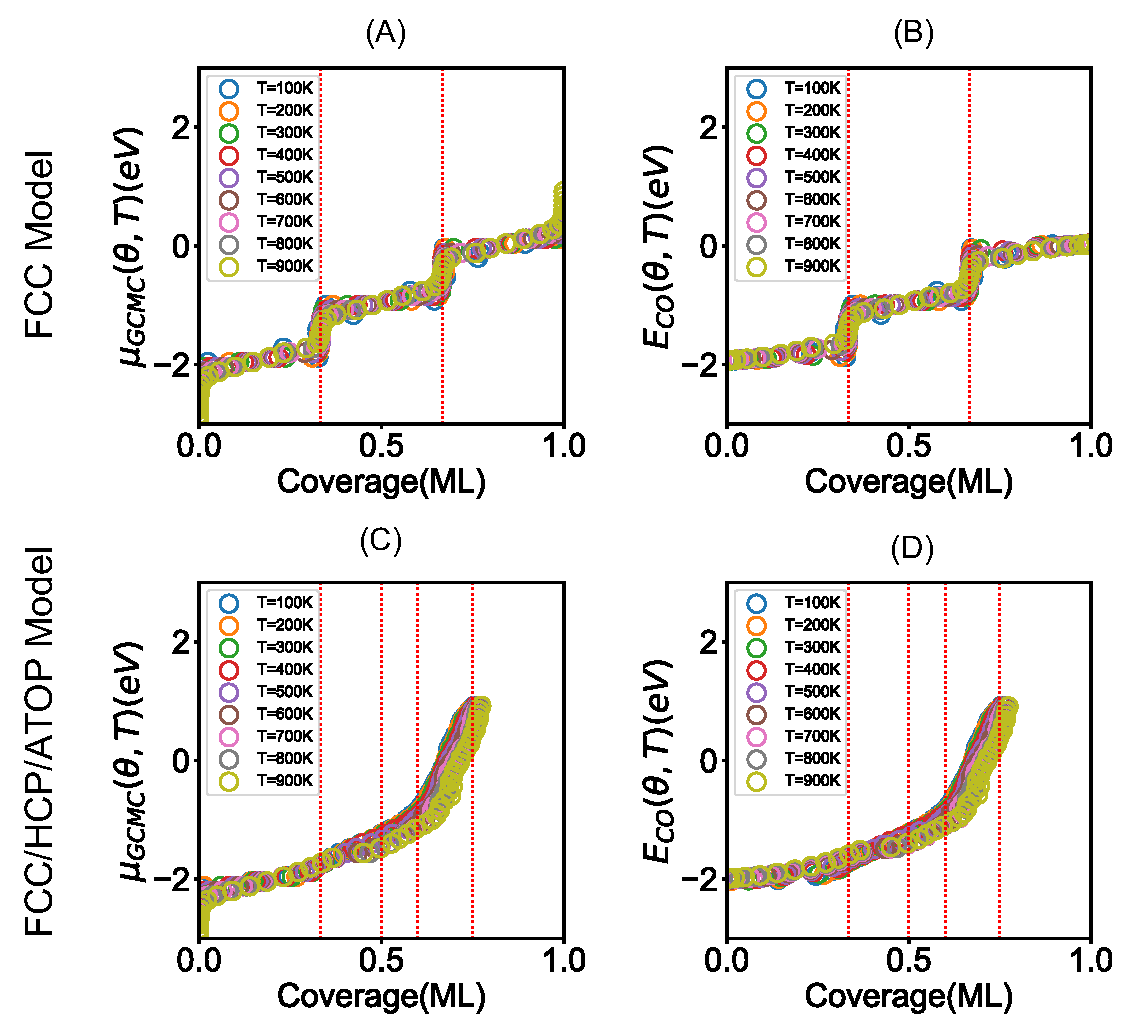
\includegraphics[width=15cm]{Figure/GCMC1.pdf}
\caption{First column: $\mu_{\ce{CO}}(\theta,T)$ vs.\ coverage for FCC model and FCC/HCP/ATOP models from top to bottom at temperature range from 100K to 900K. Last column: $E_{\ce{CO}}(\theta,T)$ vs.\ coverage for the same models.}
\label{sumgcmc}
\end{figure}

\begin{enumerate}
\item GCMC simulations were performed from 100K to 900K on the one-site and three-site CE models. Results are shown in Figure \ref{sumgcmc} A and C, plotted as $\mu_{\ce{GCMC}}(\theta,T)$ vs.\ $\theta_{\text{CO}}$. 
\item The chemical potential diverges in the limits of 0 and 1~ML, reflecting the divergence of Eq.~\ref{entropy_n_meanfield} in those limits. The one-site model (Figure~\ref{sumgcmc} A) retains the 0~K stair-step pattern smeared out at the boundaries of each ground states. The three site model (Figure~\ref{sumgcmc} C) shows a qualitatively different gradual rise in chemical potential to approximately 0.6~ML, followed by a sharper rise from 0.6 to 0.75 ML.
\item Figure \ref{sumgcmc} B and D shows $\bar{E}_{\ce{CO}}(\theta,T)$ vs.\ $\theta$ extracted using Eq.~\ref{gcmc}. Subtraction of the mean-field configurational entropy eliminates the divergences at the extremes of coverage and damps the rise in energy at intermediate coverage. Further, the sharp discontinuities present in the 0~K differential binding energies are smeared out at finite temperature. Figure \ref{sumgcmc} B and D show that the differential binding energies extracted this way are only weakly temperature dependent. 
\end{enumerate}

\clearpage
\subsubsection*{Coverage-Dependent Binding Energy Models }
\textbf{FCC Model} 

\begin{figure} [h]
\centering
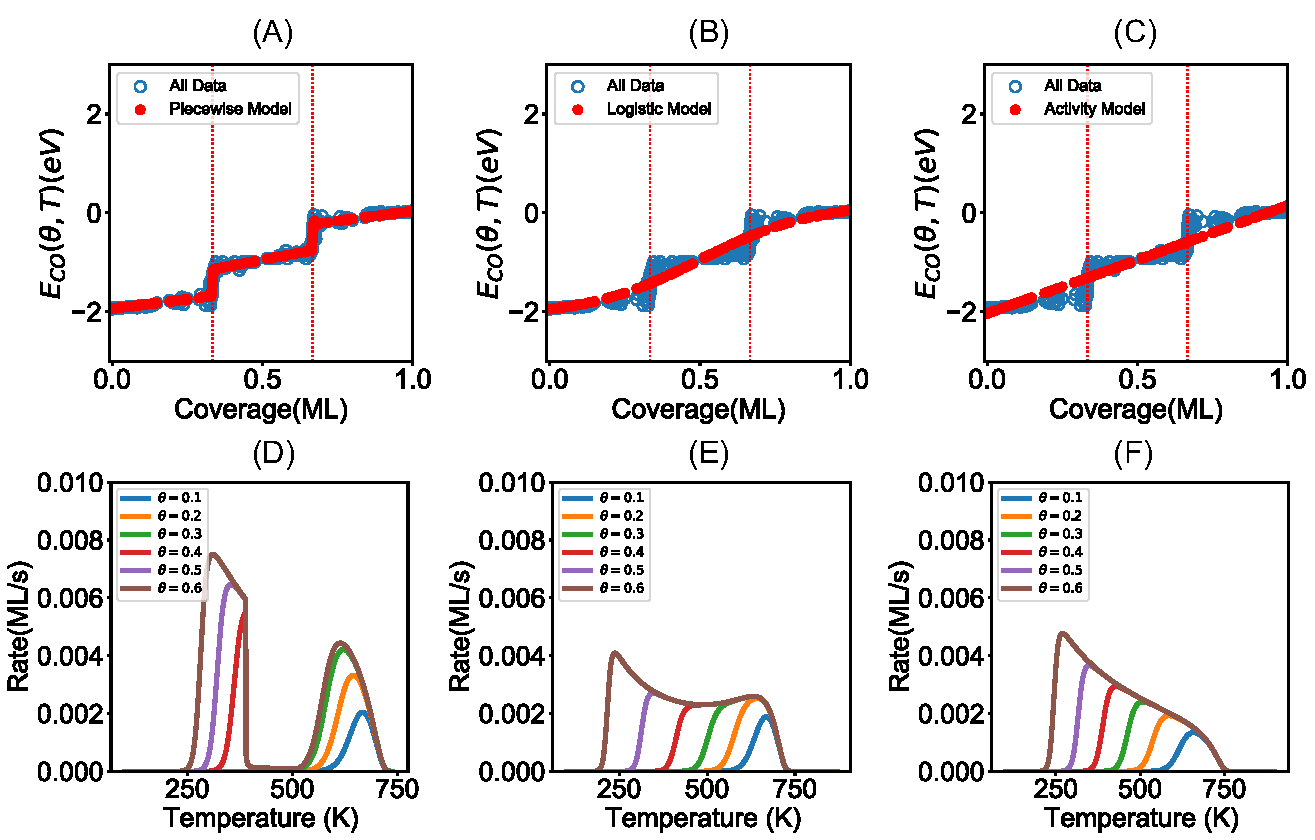
\includegraphics[width=15cm]{Figure/1function.pdf}
\caption{First column: piecewise model fit to all data point and correspond TPD plot. Second column: logistic model fit to all data point and correspond TPD plot. Third column: activity model fit to all data point and correspond TPD plot.}
\label{1func}
\end{figure}

\begin{table} [h]
\caption{Analytical Fitting Result for FCC Model }
\centering
\begin{tabular} {c c c c}
\toprule
Model & R$^2$&MAE&MSE\\
\midrule
Piecewise     &0.977 &0.0397&0.00391 \\
\\
Logistic  & 0.958 &0.106&0.0218 \\
\\
Activity  & 0.938 &0.145&0.0323 \\
\bottomrule
\end{tabular}
\label{1sitefit}
\end{table}

\begin{enumerate}
\item Figure \ref{1func} D has two different peak region below 400K and around 700K, which represent different binding energy when coverage above and below 0.3 ML.  Figure \ref{1func} E has gradually changed shape that with initial $\theta$ increasing. Clear peak is about 700K at low coverage. Figure \ref{1func} F shows peak temperature shift lower when initial $\theta$ increase, indicate that binding energy keep decreasing. Although piecewise model has the highest R$^2$ value and lowest MAE and MSE, but TPD plot did not consistent with experimental TPD \cite{Guo1989}, it suggest that one site model is insufficient to simulate real TPD.
\end{enumerate}
\clearpage

\subsubsection*{FCC/HCP/ATOP Model}

\begin{figure} [h]
\centering
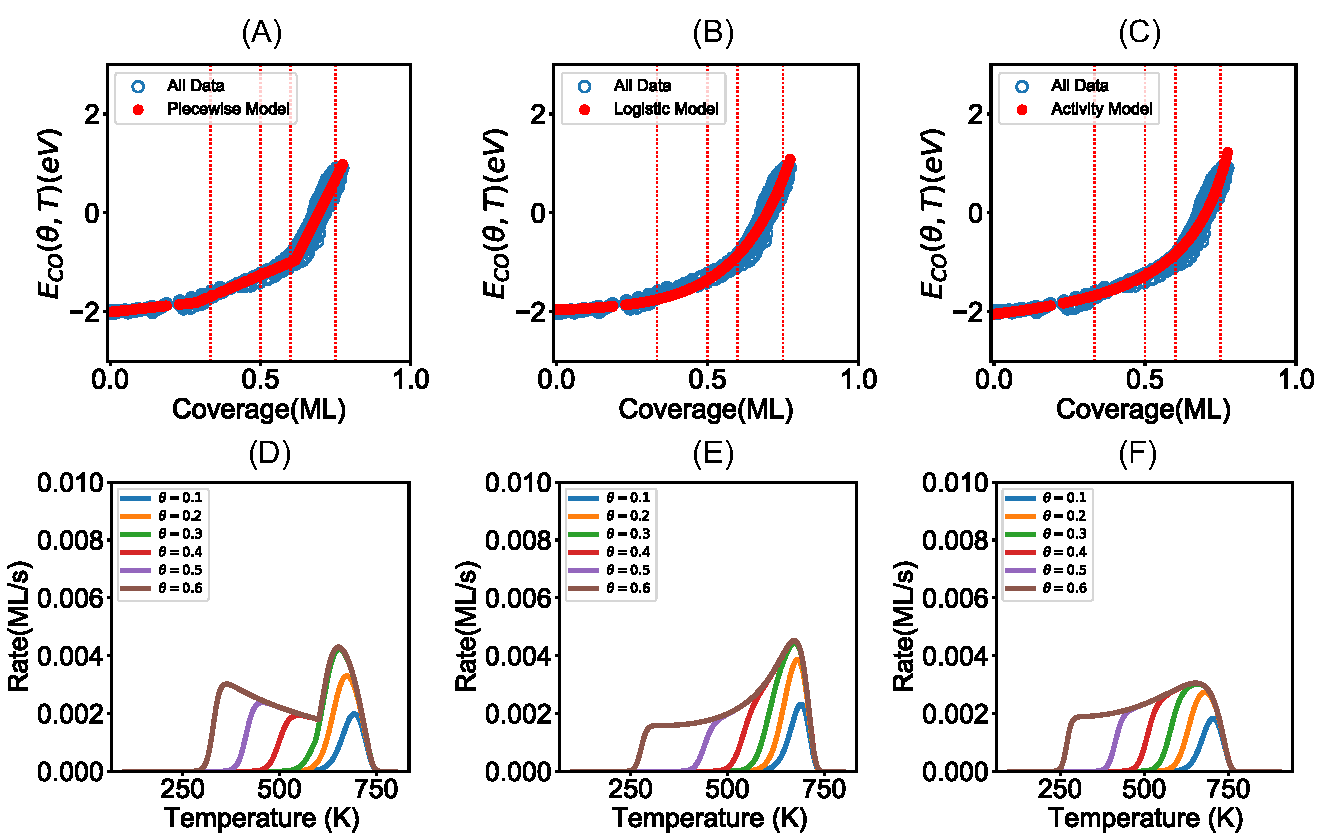
\includegraphics[width=15cm]{Figure/3function.pdf}
\caption{First column: linear model fit to all data point and correspond TPD plot. Second column: logistic model fit to all data point and correspond TPD plot. Third column: activity model fit to all data point and correspond TPD plot.}
\label{3func}
\end{figure}

\begin{table} [h]
\caption{Analytical Fitting Result for FCC/HCP/ATOP Model }
\centering
\begin{tabular} {c c c c}
\toprule
Model & R$^2$&MAE&MSE\\
\midrule
Piecewise     &0.975 &0.110&0.00224 \\
\\
Logistic  & 0.970 &0.126&0.0265\\
\\
Activity  & 0.968 &0.126&0.0285 \\
\bottomrule
\end{tabular}
\label{3sitefit}
\end{table}

\begin{enumerate}
\item From Table \ref{3sitefit}, three model have similar R$^2$ value, but piecewise have lowest MAE and MSE value. However, simulated TPD has irregular area when intial $\theta$ above 0.3 ML.
\item Logistic and activity model have similar fitting result and logistic model TPD figure has general shape that consistent with experimental TPD. When initial $\theta$ below 0.3 ML, desorption temperature peak is around 700K. When initial $\theta$ above 0.3 ML, it has long leading edge represent gradually changed binding energy.
\item  Compare Figure \ref{3func} E and F, TPD plot largely depend on fitting model. 
\end{enumerate}

\clearpage

\subsection*{Conclusion}
\begin{enumerate}
\item Simulation result of one site model can recover DFT-computed binding energy trend, but simulated TPD plot using three analytical model cannot recover features of experimental TPD.
\item Simulation result of two site and three site model cannot follows DFT-computed binding energy trend, but simulated TPD can recover general shape and high temperature peak using logistic model. Therefore, including multi-site is necessary to recover experimental TPD.
\item Three-site model can recover high temperature peak around 700K, which higher than 500K  of experimental TPD, because DFT tend to over estimate binding energy on Pd surface. Further, accurate capture coverage-dependent binding energy can contribute to construct WGS microkinetic model.
\end{enumerate}

\clearpage
\printbibliography

\clearpage
\subsection*{Supporting Information}
\subsubsection*{FCC Model}
\begin{figure} [h]
\centering
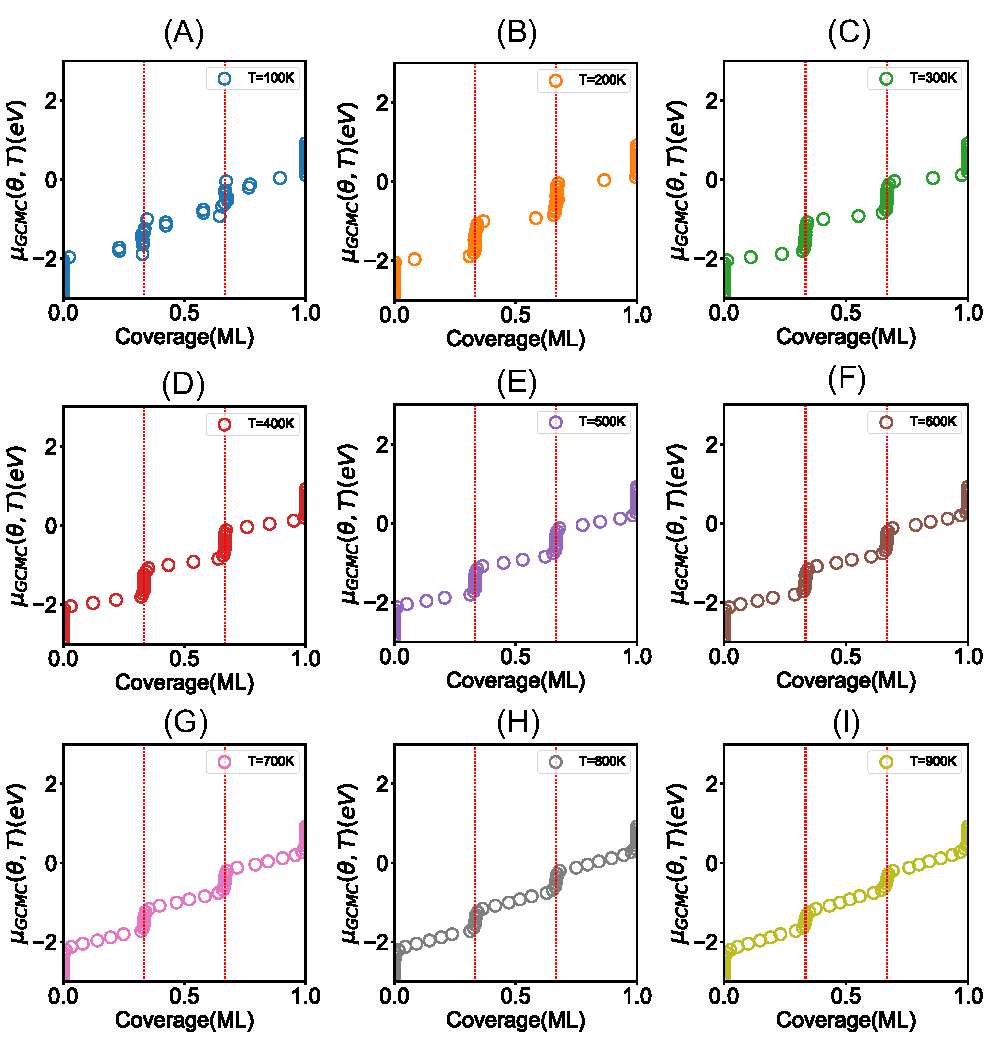
\includegraphics[width=15cm]{Figure/1Miu-T.pdf}
\caption{FCC Model simulation result of chemical potential $\mu$ vs.\ CO coverage from 100K to 900K. Red line represent ground state computed from DFT energy.}
\label{1miu}
\end{figure}

\clearpage
\begin{figure} [h]
\centering
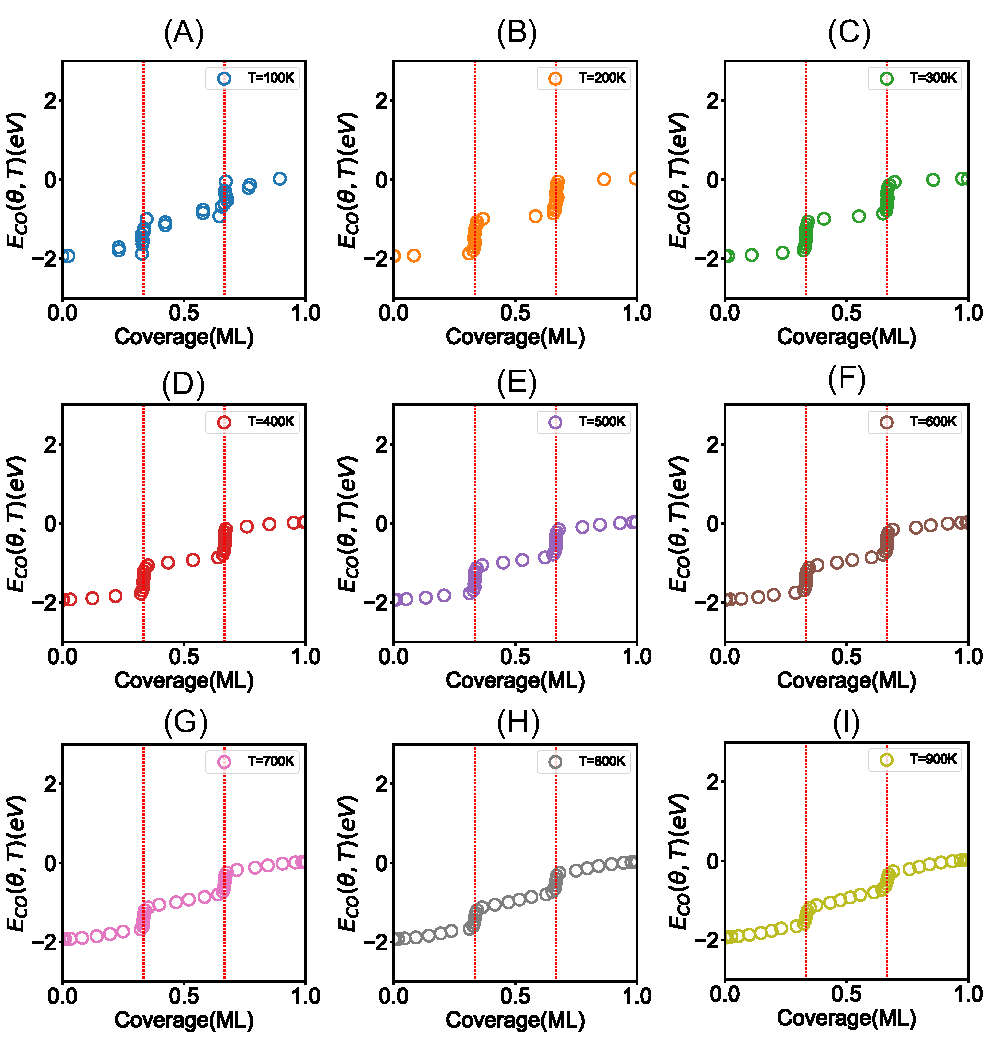
\includegraphics[width=15cm]{Figure/1E-T.pdf}
\caption{FCC Model binding energy vs.\ CO coverage from 100K to 900K after applying equation \ref{gcmc}}
\label{1E}
\end{figure}
\clearpage

\subsubsection*{FCC/HCP Model}
\begin{figure} [ht]
\centering
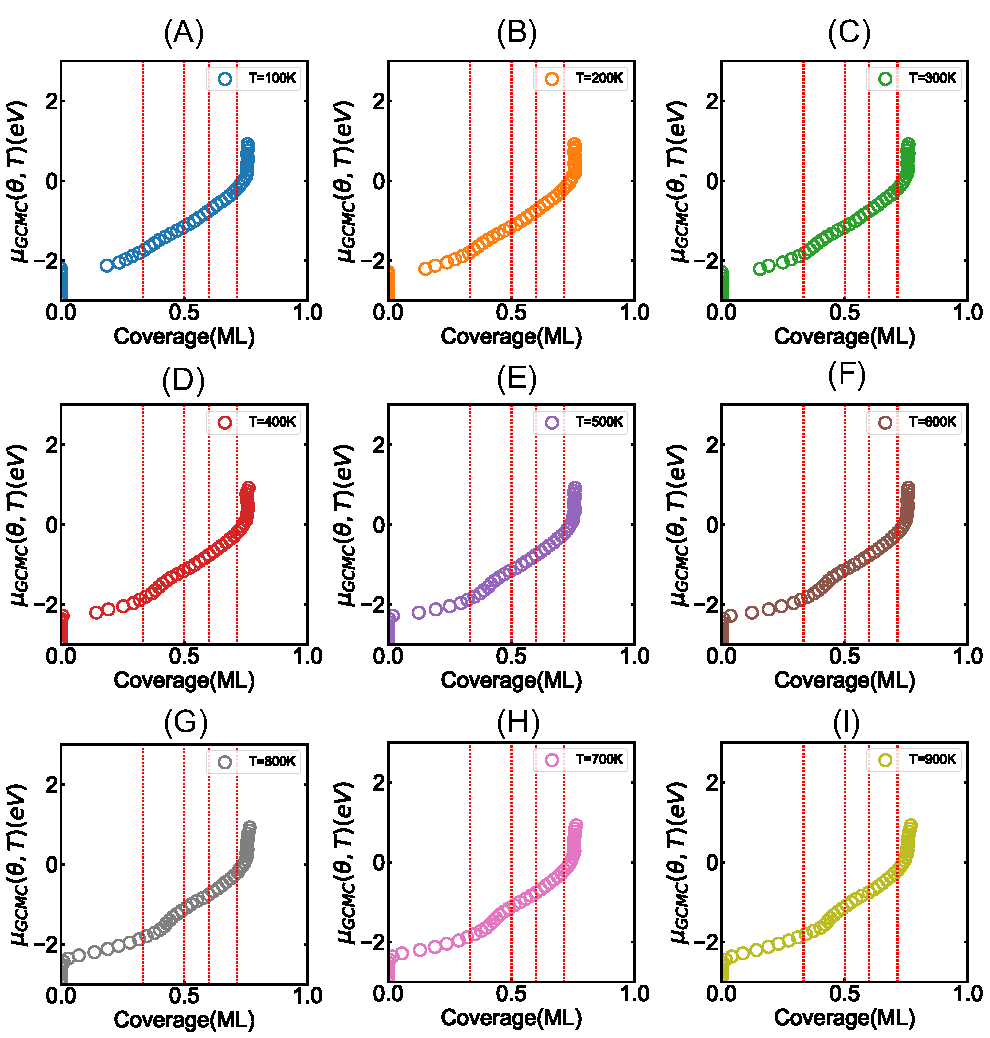
\includegraphics[width=15cm]{Figure/2Miu-T.pdf}
\caption{FCC/HCP Model simulation result of chemical potential $\mu$ vs.\ CO coverage from 100K to 900K. Red line represent ground state computed from DFT energy.}
\label{2miu}
\end{figure}
\clearpage
\begin{figure} [ht]
\centering
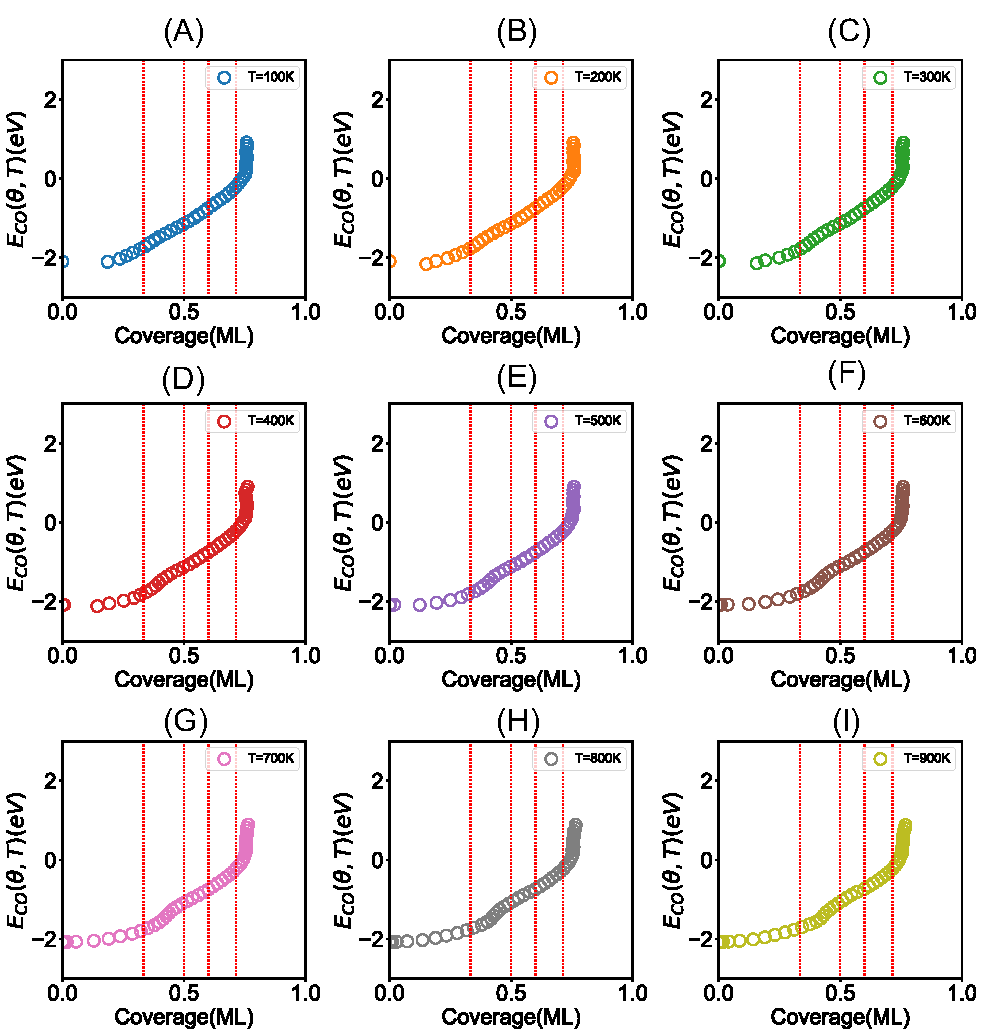
\includegraphics[width=15cm]{Figure/2E-T.pdf}
\caption{FCC/HCP Model binding energy vs.\ CO coverage from 100K to 900K after applying equation \ref{gcmc}}
\label{2E}
\end{figure}

\begin{figure} [h]
\centering
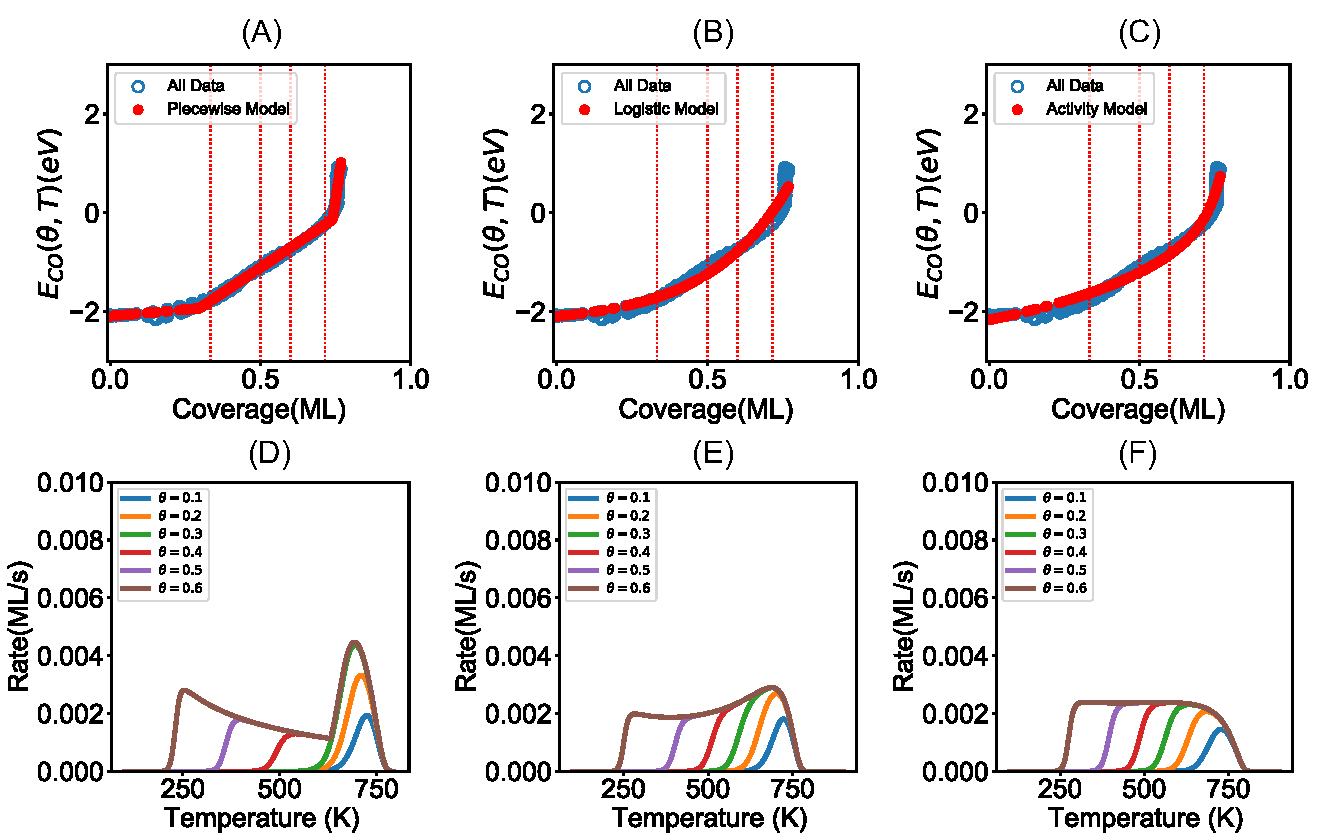
\includegraphics[width=15cm]{Figure/2function.pdf}
\caption{First column: linear model fit to all data point and correspond TPD plot. Second column: logistic model fit to all data point and correspond TPD plot. Third column: activity model fit to all data point and correspond TPD plot.}
\label{2func}
\end{figure}

\begin{table} [h]
\caption{Analytical Fitting Result for FCC/HCP Model }
\centering
\begin{tabular} {c c c c}
\toprule
Model & R$^2$&MAE&MSE\\
\midrule
Piecewise     &0.989 &0.0629&0.00987 \\
\\
Logistic  & 0.971 &0.121&0.0261 \\
\\
Activity  & 0.978 &0.118&0.0202 \\
\bottomrule
\end{tabular}
\label{2sitesimu}
\end{table}

\clearpage

\subsubsection*{FCC/HCP/ATOP Model}
\begin{figure} [ht]
\centering
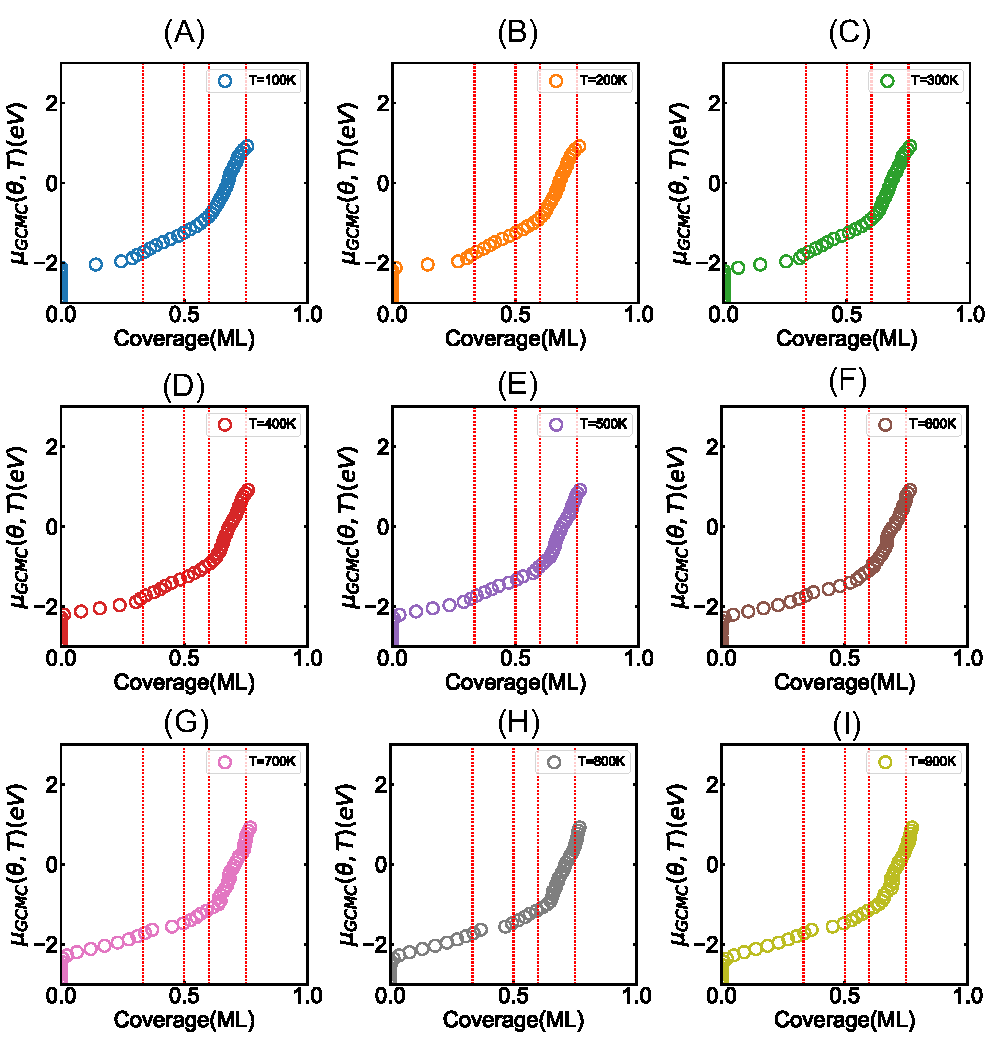
\includegraphics[width=15cm]{Figure/3Miu-T.pdf}
\caption{FCC/HCP/ATOP Model simulation result of chemical potential $\mu$ vs.\ CO coverage from 100K to 900K. Red line represent ground state computed from DFT energy.}
\label{3miu} 
\end{figure}
\clearpage

\begin{figure} [h]
\centering
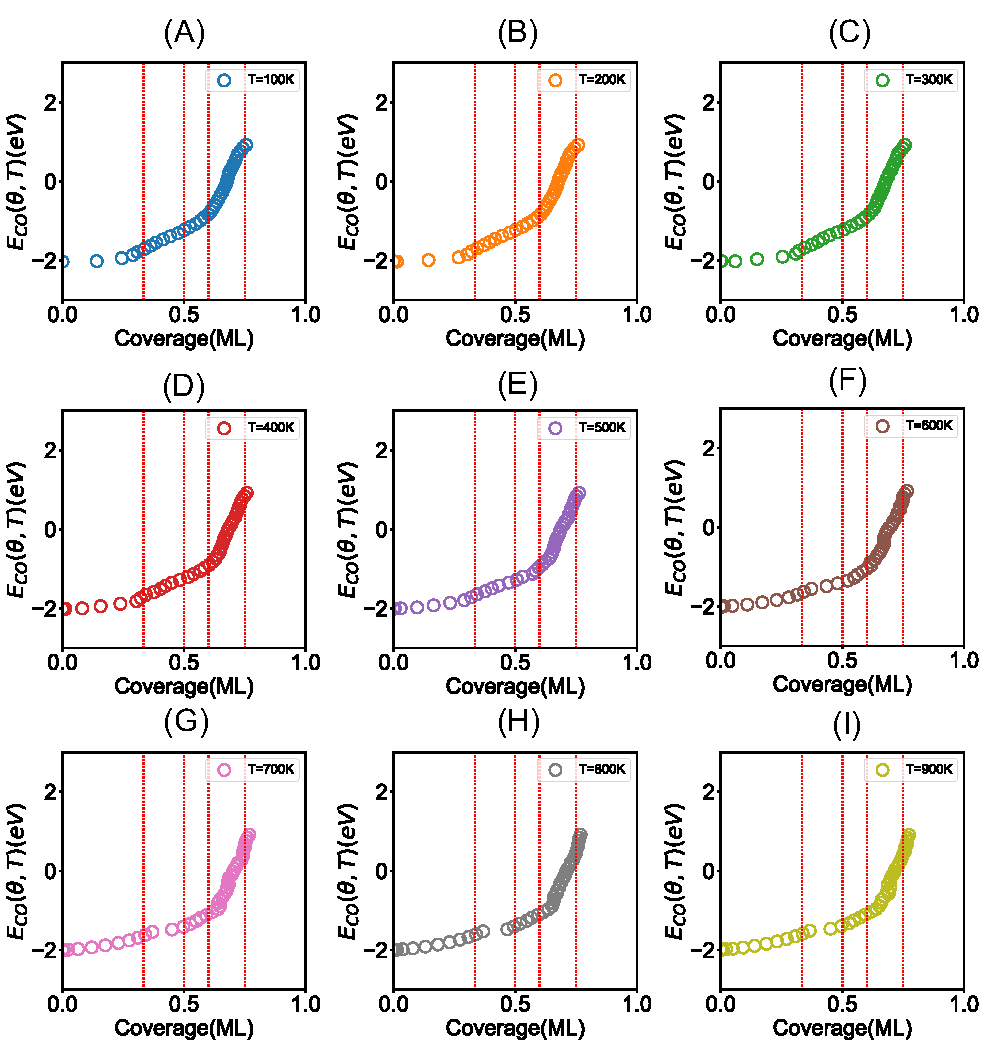
\includegraphics[width=15cm]{Figure/3E-T.pdf}
\caption{FCC/HCP/ATOP Model binding energy vs.\ CO coverage from 100K to 900K after applying equation \ref{gcmc}}
\label{2E}
\end{figure}


\end{document}